\documentclass[a4paper]{article}
\usepackage{titling}
\usepackage{authblk}
\usepackage{fancyhdr}
\usepackage[hyphens]{url}
\usepackage{hyperref}
\usepackage{rsc}
\usepackage{siunitx}
\usepackage{graphicx}
\usepackage{mhchem}
\usepackage{amsmath}
\usepackage{listings}
\usepackage{color}
\usepackage[htt]{hyphenat}
\usepackage{subcaption}

\definecolor{dkgreen}{rgb}{0,0.6,0}
\definecolor{gray}{rgb}{0.5,0.5,0.5}
\definecolor{mauve}{rgb}{0.58,0,0.82}
\graphicspath{{../figures/}}

\lstset{frame=tb,
  language=Python,
  aboveskip=3mm,
  belowskip=3mm,
  showstringspaces=false,
  columns=flexible,
  basicstyle={\ttfamily},
  numbers=none,
  numberstyle=\tiny\color{gray},
  keywordstyle=\color{blue},
  commentstyle=\color{dkgreen},
  stringstyle=\color{mauve},
  breaklines=true,
  breakatwhitespace=true,
  tabsize=3,
  postbreak=\mbox{\textcolor{red}{$\hookrightarrow$}\space},
  columns=fixed,basewidth=.5em,
}

\setcounter{section}{-1}

\title{Lecture 9: Eigenvalues and eigenvectors}
\author[1]{Dr Benjamin J. Morgan}
\author[1,2]{Dr Andrew R. McCluskey}
\affil[1]{Department of Chemistry, University of Bath, email: b.j.morgan@bath.ac.uk}
\affil[2]{Diamond Light Source, email: andrew.mccluskey@diamond.ac.uk}
\setcounter{Maxaffil}{0}
\renewcommand\Affilfont{\itshape\small}
\newcommand{\bvec}[1]{\boldsymbol{\mathbf{#1}}}
\newcommand{\norm}[1]{\left\lVert #1\right\rVert}
\newcommand{\cvec}[2]{\begin{bmatrix}#1\\#2\end{bmatrix}}
\newcommand{\tmatrix}[4]{\begin{bmatrix}#1&#2\\#3&#4\end{bmatrix}}

\pagestyle{fancy}
\fancyhf{}
\rhead{CH40208}
\lhead{\thetitle}
\rfoot{\thepage}

\begin{document}
\maketitle

\section*{Aim}
This week's session continues from last week's content on \emph{vectors} and \emph{matrices}, and how we can use Python to perform vector and matrix maths.
This week we will look at eigenvalue equations, solving these using Python, and some examples of where these come up in computational chemistry.

\section{Recap}
Key points from last week:

\subsection{Vectors}
\begin{itemize}
  \item \emph{Vectors} are properties with both \emph{magnitude} and \emph{direction} (in contrast to \emph{scalars}, which only have magnitude.)
  \item Vectors can be represented as a \emph{linear combination} of basis vectors:
    \begin{equation*}
    \bvec{v}=\sum_i c_i \phi_i.
    \end{equation*}
  e.g.\ for a two dimensional vector space with basis vectors $\bvec{i}$ and $\bvec{j}$, the column vector $\cvec{2}{3}$ describes a vector $2\bvec{i}+3\bvec{j}$.
  \item In Python, we can represent vectors using one-dimensional numpy arrays, e.g.
  \begin{lstlisting}
  >>> import numpy as np
  >>> v = np.array([2, 3])
  >>> print(v)
  [2, 3]
  \end{lstlisting}
  \item numpy arrays behave like vectors for addition and scalar multiplication:
  \begin{lstlisting}
  >>> print(a*2)
  [4, 6]
  >>> u = np.array([3, 5])
  >>> print(u + v)
  [5, 8]
  >>> print(u - v)
  [1, 2]
  \end{lstlisting}
  \item The dot product and cross product operations are provided as part of numpy:
  \begin{lstlisting}
  >>> print(np.dot(u, v))
  21
  >>> print(np.cross(u, v))
  -1
  \end{lstlisting}
\end{itemize}

\subsection{Matrices}
\begin{itemize}
  \item Matrices describe \emph{linear transformations}: we generate a new set of basis vectors as a linear combination of the original basis vectors. e.g.\ in two dimensions, the matrix $\bvec{M}=\begin{bmatrix}a & c\\b & d\end{bmatrix}$ describes the basis transformation
  \begin{eqnarray}
  \bvec{i} & \to & \bvec{i^\prime}\\
  \bvec{j} & \to & \bvec{j^\prime}.
  \end{eqnarray}
  where
  \begin{eqnarray}
  \bvec{i^\prime} & = & a\times\bvec{i} + b\times\bvec{j} \\
  \bvec{j^\prime} & = & c\times\bvec{i} + d\times\bvec{j}.
  \end{eqnarray}
  i.e.\ the \emph{columns} of the matrix $\bvec{M}$ describe the transformation of the vectors $\cvec{1}{0}$ and $\cvec{0}{1}$.
  \item We can calculate the effect of a matrix $\bvec{M}$ operating on a vector $\bvec{v}$ by calculating the effect of the matrix operating on the basis vectors $\bvec{i}$ and $\bvec{j}$ and then multiplying these by the vector elements, e.g.
  \begin{eqnarray}
  \bvec{v^\prime} & = & \bvec{M}\cdot\bvec{v}\\
  & = & \begin{bmatrix}a & c\\b & d\end{bmatrix}\cdot\cvec{v_1}{v_2} \\
  & = & v_1\cvec{a}{b} + v_2\cvec{c}{d} \\
  & = & v_1\times\bvec{i^\prime} + v_2\times\bvec{j^\prime}.
  \end{eqnarray}
  \item In Python, we can represent vectors using one-dimensional numpy arrays, e.g.
  \begin{lstlisting}
  >>> M = np.array([[1, 2],
                      [-1, 1]])
  >>> print(M)
  [[1 2]
   [-1 1]]
  \end{lstlisting}
  \item Matix--vector multiplication can be performed using \texttt{np.matmul()}:
  \begin{lstlisting}
  >>> print(np.matmul(M,v))
  [8, 1]
  \end{lstlisting}
  which gives the same result as a sum over vector elements times transformed basis vectors (matrix columns), using array slicing (see week ?):
  \begin{lstlisting}
  >>> print(v[0]*M[:,0] + v[1]*M[:,1])
  [8, 1]
  \end{lstlisting}
  \item The combined effect of one matrix operation followed by a second can be described by a single matrix. The new matrix is generated by multiplying the two original matrices together. In Python we can use the \texttt{np.matmul()} function for matrix multiplication:
  \begin{equation*}
  \bvec{M}  =  \begin{bmatrix}2&1\\1&2\end{bmatrix};
  \end{equation*}
  \begin{equation*}
  \bvec{N}  =  \begin{bmatrix}0&1\\1&1\end{bmatrix}.
  \end{equation*}
  \begin{eqnarray*}
  \bvec{P}& = & \bvec{M}\cdot\bvec{N} \\
          & = & \begin{bmatrix}2&1\\1&2\end{bmatrix}\cdot\begin{bmatrix}0&1\\1&1\end{bmatrix} \\
          & = & \begin{bmatrix}1&3\\2&3\end{bmatrix}.
  \end{eqnarray*}
  \item The reverse or \emph{inverse} of a matrix operation, $\bvec{M}$ is described by the matrix inverse $\bvec{M}^{-1}$. We can compute this in Python using \texttt{np.linalg.inv(M)}.
\end{itemize}
\pagebreak
\section{Eigenvalues and Eigenvectors}
We have seen that a matrix $\bvec{M}$ operating on a vector $\bvec{v}$ produces a new vector $\bvec{v^\prime}$:
\begin{equation*}
\bvec{v}^\prime = \bvec{M}\cdot\bvec{v}.
\end{equation*}
In general the matrix $\bvec{M}$ can change both the magnitude and direction of the vectors $\bvec{v}\to\bvec{v^\prime}$. 

Consider the matrix $\bvec{M}=\begin{bmatrix}2&1\\1&2\end{bmatrix}$. This gives the linear transformation shown in Figure~\ref{fig:matrix_transformation}. We can also visualise this transformation by considering the effect on a set of vectors with length $1$ and different directions; shown in Figure~\ref{fig:matrix_transformation_unit_circle}. Now we see that the effect of the matrix transformation is to transform a unit circle into an ellipse.
\begin{figure}[tb]
  \centering
  \resizebox{12cm}{!}{\includegraphics*{matrix_transformation.pdf}} %
    \caption{\label{fig:matrix_transformation}CAPTION}
\end{figure}

\begin{figure}[tb]
  \centering
  \resizebox{12cm}{!}{\includegraphics*{matrix_transformation_unit_circle.pdf}}
    \caption{\label{fig:matrix_transformation_unit_circle}The effect of the matrix $\bvec{M}$ is to transform the unit circle (left) into an ellipse (right).}
\end{figure}

The major and minor axes of this ellipse (given by the longest and shortest transformed vectors) lie along $\cvec{1}{1}$ and $\cvec{-1}{1}$, respectively. If we compare these transformed vectors to the corresponding \emph{original} vectors we see that the effect of $\bvec{M}$ operating on these two vectors is only to scale them. Their directions have not changed (Figure~\ref{fig:ellipse_major_minor_axes_transformation}). Mathematically, this means
\begin{eqnarray*}
\bvec{v^\prime}&=&\bvec{M}\cdot\bvec{v} \\
s\bvec{v}&=&\bvec{M}\cdot\bvec{v}.
\end{eqnarray*}
i.e. operating on $\bvec{v}$ by $\bvec{M}$ gives the \emph{same vector} $\bvec{v}$ back, times a scalar, $s$. This only happens for these two ``special'' vectors, which we call the \emph{eigenvectors} of the matrix $\bvec{M}$. The scalar values $s$ are the \emph{eigenvalues} of the matrix $\bvec{M}$.

\begin{figure}[tb]
  \centering
  \resizebox{12cm}{!}{\includegraphics*{ellipse_major_minor_axes_transformation.pdf}} %
    \caption{\label{fig:ellipse_major_minor_axes_transformation}Left: The two vectors corresponding to the major and minor axes of the ellipse in Figure~\ref{fig:matrix_transformation_unit_circle}. Right: The same two vectors \emph{before} the transformation. Both of these vectors have the same direction before and after the transformation by $\bvec{M}$ and are \emph{eigenvectors} of $\bvec{M}$.}
\end{figure}

We can calcuate the eigenvalues and eigenvectors of a matrix using texttt{np.linalg.eig()}\footnote{\url{https://docs.scipy.org/doc/numpy/reference/generated/numpy.linalg.eig.html}}:
\begin{lstlisting}
>>> print(np.linalg.eig(M))
(array([3., 1.]), array([[ 0.70710678, -0.70710678],
       [ 0.70710678,  0.70710678]]))
\end{lstlisting}
This returns two arrays. The first array contains the eigenvalues of $\bvec{M}$, and the second array contains the eigenvectors of $\bvec{M}$.
\begin{lstlisting}
>>> print(np.linalg.eig(M)[0])
[3., 1]
>>> print(np.linalg.eig(M)[1])
[[ 0.70710678 -0.70710678]
 [ 0.70710678  0.70710678]]
\end{lstlisting}
Note that the eigenvectors are returned as a matrix. Each of the \emph{columns} of this matrix correspond to one of the eigenvectors. We can see that for the matrix $\bvec{M}=\tmatrix{2}{1}{1}{2}$ we get one eigenvector $\cvec{0.70710678}{0.70710678}$ with eigenvalue $3$, and a second eigenvector $\cvec{-0.70710678}{\phantom{-}0.70710678}$ with eigenvalue $1$.

Calculating eigenvalues and eigenvectors is useful in a number of chemistry applications, for example:
\begin{itemize}
 \item Describing the rotational motions of molecules---finding principal axes of rotation and principal moments of inertia (eigenvectors and eigenvalues of the inertia matrix).
 \item Describing the vibrational motions of molecules---finding normal modes (eigenvectors of the dynamical matrix and their associated frequencies (eigenvectors and eigenvalues of the dynamical matrix).
 \item Solving the time-independent Schr\"{o}dinger equation $H\Psi=E\Psi$, which is an eigenvalue equation, to find molecular orbitals and their corresponding energies (eigenvectors and eigenvalues of the Hamiltonian matrix).
\end{itemize}

\subsection{Key ideas}
\begin{itemize}
  \item A two-dimensional matrix transforms a unit circle into an ellipse.
  \item A vector that does not change direction under the operation $\bvec{M}$ is an \emph{eigenvector} of $\bvec{M}$. The scaling factor of this vector is the corresponding \emph{eigenvalue}.
\end{itemize}

\section{Principal Rotation Axes and Principal Moments of Intertia}
The rotational energy levels of a molecule depend upon the molecule's moments of inertia, making these important molecular quantities for interpreting rotational spectra, or for calculating the rotational partition function:
\begin{equation}
q_\mathrm{rot} = \frac{\pi^{\frac{1}{2}}}{\sigma}\left(\frac{k_\mathrm{B}T}{hcA}\right)^\frac{1}{2}\left(\frac{k_\mathrm{B}T}{hcB}\right)^\frac{1}{2}\left(\frac{k_\mathrm{B}T}{hcC}\right)^\frac{1}{2},
\end{equation}
where $A$, $B$, and $C$ and the \emph{principal moments of inertia} of a non-linear molecule.

Moments of inertia, described by $\bvec{I}$, describe how a rigid body responds to angular acceleration, and are analogous to intertial mass for linear acceleration:
\begin{align*}
\bvec{F} = m\bvec{a} && \bvec{\tau} = \bvec{I} \bvec{\alpha} \\
\bvec{p} = m\bvec{v} && \bvec{h}    = \bvec{I}\bvec{\omega} 
\end{align*}

If we focus on angular momentum, then for a one-dimensional problem, where rotation occurs around a single axis (e.g. for a diatomic molecule), $\bvec{\omega}$ and $\bvec{h}$ are scalars and $\bvec{I}$ is also a scalar:
\begin{equation*}
h = I\omega
\end{equation*}
For a rigid diatomic molecule the moment of inertia, $I$, is given by
\begin{equation*}
I = \sum_i m_i r_i^2
\end{equation*}
where $r_i$ is the distance of each atom from the centre of mass. This is often written in terms of the \emph{reduced mass} of the molecule, $\mu$:
\begin{equation*}
I = \mu r^2
\end{equation*}
where $r$ is the molecular bond length.

In three dimensions, however, $\bvec{\omega}$, and $\bvec{h}$ are \emph{vectors}, and are not required to have the same orientation. The quantity $\bvec{I}$, which translates one vector into another vector, is therefore a \emph{matrix}, called the \emph{intertia matrix}:
\begin{equation*}
\begin{bmatrix}l_x\\l_y\\l_z\end{bmatrix} = 
\begin{bmatrix} 
I_{xx} & I_{xy} & I_{xz} \\
I_{yx} & I_{yy} & I_{yz} \\
I_{zx} & I_{zy} & I_{zz} 
\end{bmatrix}
\cdot
\begin{bmatrix}\omega_x\\\omega_y\\\omega_z\end{bmatrix}.
\end{equation*}
where the \emph{diagonal} elements (called ``moments of inertia'') are similar to the one-dimensional definition, e.g.
\begin{eqnarray*}
I_{xx} = \sum_i m_i(y_i^2+z_i^2), \\
I_{yy} = \sum_i m_i(x_i^2+z_i^2), \\
I_{zz} = \sum_i m_i(x_i^2+y_i^2);
\end{eqnarray*}
but the \emph{off-diagonal} elements (called ``products of inertia'') must also be included:
\begin{eqnarray*}
I_{xy} = \sum_i m_ix_iy_i
\end{eqnarray*}
etc.

Having non-zero off-diagonal elements in the intertia matrix makes working with angular motion in 3D more complicated than in 1D. It is often useful therefore to seek a simpler form for $\bvec{I}$ that gives a more intuitive description of molecular rotational properties.

Each of the elements of $\bvec{I}$ contains terms like 
$x_i^2$ 
or $xy$, where $x$, $y$, and $z$ are distances of atoms along each direction from the centre of mass. The values of each element of $\bvec{I}$ therefore depend on the relative orientation of the $\left\{x,y,z\right\}$ coordinate system and the molecule. Choosing a differently oriented coordinate system changes the $x$, $y$, and $z$ coordinates of each atom, and changes the values of the elements of $\bvec{I}$. We might therefore ask: is there a choice of molecular orientation / coordinate orientation where the off-diagonal elements of $\bvec{I}$ are all zero?

If this were the case, our angular momentum equation would now be:
\begin{equation*}
\begin{bmatrix}l_x\\l_y\\l_z\end{bmatrix} = 
\begin{bmatrix} 
I_{xx} & 0 & 0 \\
0 & I_{yy} & 0 \\
0 & 0 & I_{zz} 
\end{bmatrix}
\cdot
\begin{bmatrix}\omega_x\\\omega_y\\\omega_z\end{bmatrix}.
\end{equation*} 
and each component of $\bvec{l}$ would be directly proportional to the corresponding component of $\bvec{w}$. The ``products of inertia'' now do not appear, and we can describe the rotational properties of the molecule by specifying the three moments of inertia.

It turns out that such a coordinate system can be found, and it corresponds to choosing the \emph{eigenvectors} of $\bvec{I}$ as our basis vectors. Let us suppose that we have found the eigenvalues, $\lambda_i$, and eigenvectors, $\bvec{v}_i$, of $\bvec{I}$. This gives us three eigenvalue equations:
\begin{eqnarray*}
\lambda_1 \bvec{v}_1 & = & \bvec{I}\cdot\bvec{v}_1 \\
\lambda_2 \bvec{v}_2 & = & \bvec{I}\cdot\bvec{v}_2 \\
\lambda_3 \bvec{v}_3 & = & \bvec{I}\cdot\bvec{v}_3.
\end{eqnarray*}
Let us now express our angular velocity vector $\bvec{\omega}$ using these eigenvectors as a basis:
\begin{equation*}
\bvec{\omega} = c_1\bvec{v}_1 + c_2\bvec{v}_2 + c_3\bvec{v}_3.
\end{equation*} 
And then the effect of the matrix $\bvec{I}$ operating on $\bvec{\omega}$:
\begin{eqnarray*}
\bvec{I}\cdot\bvec{\omega} & = & c_1\bvec{I}\cdot\bvec{v}_1 + c_2\bvec{I}\cdot\bvec{v}_2 + c_3\bvec{I}\cdot\bvec{v}_3 \\
& = & c_1\lambda_1\bvec{v}_1 + c_2\lambda_1\bvec{v}_2 + c_3\lambda_1\bvec{v}_3.
\end{eqnarray*}
which can be rewritten in matrix form as
\begin{eqnarray*}
\bvec{I}\cdot\bvec{\omega} & = & 
\begin{bmatrix} 
\lambda_1 & 0 & 0 \\
0 & \lambda_2 & 0 \\
0 & 0 & \lambda_3
\end{bmatrix}
\cdot
\begin{bmatrix}c_1\\c_2\\c_3\end{bmatrix} \\
& = & \begin{bmatrix} 
\lambda_1 & 0 & 0 \\
0 & \lambda_2 & 0 \\
0 & 0 & \lambda_3
\end{bmatrix}
\cdot
\bvec{\omega}
\end{eqnarray*}
This gives the simplified form that we wanted, \emph{if} we use the eigenvectors of $\bvec{I}$ as our basis vectors, i.e.\ as our coordinate system vectors. The eigenvectors of the inertia matrix are called the \emph{principal rotation axes} of our molecule, and the corresponding eigenvalues are the \emph{principal moments of inertia}.

For a molecular in an arbitrary orientation, we can therefore calculate the principal moments of inertia by finding the eigenvalues of the inertia matrix. The corresponding eigenvectors give us the principal rotation axes, which are often used to define a ``natural'' coordinate system for the molecule.

\subsection{Rotating molecules onto their principal rotation axes}.
If the principal rotation axes of a molecule define a natural coordinate system for that molecule, are we able to rotate an arbitrarily oriented molecule onto this coordinate system? The answer is yes, and it combines the rotataion matrices from week 8 with the eigenvectors discussed this week.

For a given molecular rotation, the basis vectors $\bvec{i}$, $\bvec{j}$, and $\bvec{k}$ point along $x$, $y$, and $z$ respectively. But we would like to rotate our molecule (or equivalently to rotate the coordinate system) so that $x$, $y$, and $z$ point along the principal rotation axes of the molecule. This is equivalent to \emph{transforming} our coordinate system so that $\bvec{i}$, $\bvec{j}$, and $\bvec{k}$ are aligned with the eigenvectors of the inertia matrix $\bvec{I}$ (for the original coordinate system). Remember that a matrix transformation maps the original basis vectors onto the columns of the matrix. To map $\bvec{i}$, $\bvec{j}$, and $\bvec{k}$ onto $\bvec{v}_1$, $\bvec{v}_2$, and $\bvec{v}_3$ we operate on the vector coordinates of the atoms in the molecule with a matrix composed of $\bvec{k}$ onto $\bvec{v}_1$, $\bvec{v}_2$, and $\bvec{v}_3$ as columns.

\vspace{\baselineskip}
\begin{center}
  \noindent\fbox{%
      \begin{minipage}{0.9\textwidth}%
          \vspace{0.15\baselineskip}
      \subsubsection*{Exercise}
          Today's exercise is to calculate principal moments of inertia and principal rotation axes of a series of molecules, and then to rotate these molecules so that they the principal axes are aligned with $\left\{x, y, z\right\}$.

          The coordinates of each molecule can be downloaded from Moodle, where you will also find a \texttt{visualisation2.py} module that contains some code for visualising your molecules and their orientations.

          In terms of planning your code, you want to be able to perform the following sequence of steps:
          \begin{enumerate}
            \item Each file contains data in the format $\left\{x, y, z, m\right\}$ for each atom, where $m$ is the atomic mass of that atom. You will first want to read this in, and extract the atomic coordinates and masses.
            \item Construct the inertia matrix $\bvec{I}$.
            \item Calculate the eigenvalues and eigenvectors of $\bvec{I}$.
            \item Operate on your atomic coordinates to generate new coordinates, with the molecular principal axes aligned with $\left\{x, y, z\right\}$.
            \item Use the \texttt{visualisation.show()} function to look at your rotated molecules. Do these look how you would expect from what you know about molecular symmetry?
          \end{enumerate}
        
      \end{minipage}
    }
\end{center}

% \section{Vectors}
% Many problems in chemistry and physics involve working with \emph{vector} quantities. A common definition of a vector in a physics context is a quantity with both \emph{magnitude} and \emph{direction}; for example, the positions or velocities of atoms, or the forces acting on atoms within a molecule.

% \subsection{Example 1: Atomic positions}
% Defining atomic positions requires three pieces of information: the location of a reference position, called the \emph{origin}, the distance of each atom from the origin, and the direction we move from the origin to reach each atom. Positions are therefore \emph{vector} quantities (Fig.~\ref{fig:position_vectors}).
% \begin{figure*}
%   \centering
%   \begin{subfigure}[t]{0.475\textwidth}
%     \centering
%     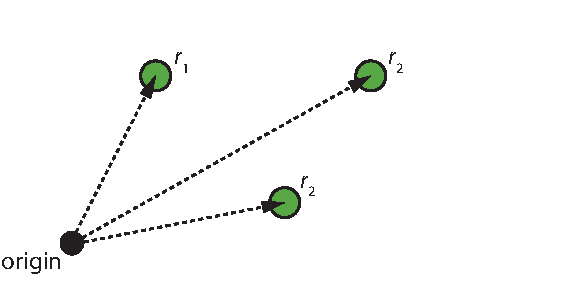
\includegraphics[width=\textwidth]{position_vectors_1}
%     \caption[Network2]%
%       {{\small Defining atomic positions requires knowing both distance and direction with respect to some reference \emph{origin}.}}    
%     \label{fig:position_vectors_1}
%   \end{subfigure}
%   \hfill
%   \begin{subfigure}[t]{0.475\textwidth}  
%     \centering 
%     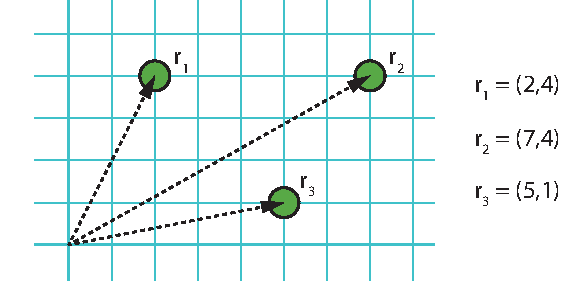
\includegraphics[width=\textwidth]{position_vectors_2}
%   \caption[]%
%       {{\small Describing positions using Cartesian coordinates, i.e.\ $(x,y)$ coordinates in two dimensions, or $(x,y,z)$ in three dimensions.}}    
%     \label{fig:position_vectors_2}
%   \end{subfigure}
%   \vskip\baselineskip
%   \begin{subfigure}[t]{0.475\textwidth}   
%     \centering 
%     \includegraphics[width=\textwidth]{position_vectors_3}
%     \caption[]%
%       {{\small The choice of coordinate system implicitly defines \emph{basis} vectors, $\bvec{i}$ and $\bvec{j}$. Any position can be expressed as a linear combination of these basis vectors.}}    
%     \label{fig:position_vectors_3}
%   \end{subfigure}
%   \quad
%   \begin{subfigure}[t]{0.475\textwidth}   
%      \centering 
%      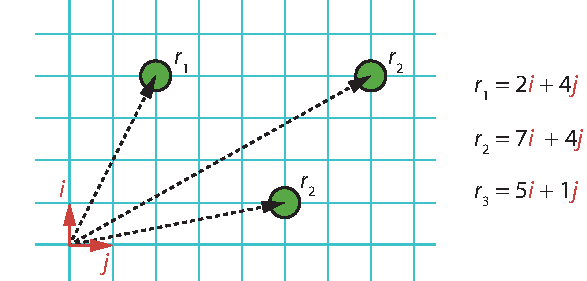
\includegraphics[width=\textwidth]{position_vectors_4}
%      \caption[]%
%        {{\small The $(x,y)$ coordinates given in \ref{fig:position_vectors_2} are the coefficients used to define each position in the basis $(\bvec{i},\bvec{j})$.}}    
%      \label{fig:position_vectors_4}
%    \end{subfigure}
%  \caption
%    {} 
%  \label{fig:position_vectors}
% \end{figure*}
% A common choice for describing atomic positions is to use Cartesian coordinates, i.e.~$(x,y)$ in two dimensions, or $(x,y,z)$ in three dimensions \footnote{A good choice of coordinate system depends on the problem at hand, and Cartesian coordinated may not always be easiest to work with. For example, problems with spherical symmetry, such as describing atomic orbitals, will often be simpler when expressed in spherical coordinates $(r, \phi, \theta)$.}; this will be familiar from the interatomic distances (week 2) and molecular rotation (week 4) problems. In two dimensions, any position can be described by giving both the $x$ coordinate and the $y$ coordinate. Using the language of vectors, this choice of $x$ and $y$ coordinates defines a pair of \emph{basis} vectors, which we will denote $\bvec{i}$ and $\bvec{j}$ 
% \footnote{Vectors are usually distinguished from scalar variables by using upright bold text, e.g.~$\bvec{r}$ (used here) or an accenting arrow, e.g.~$\vec{r}$. The components of a vector can be given as a list, e.g.~$(1,2)$, or as a column vector, e.g.~$\begin{bmatrix}1\\2\end{bmatrix}$. These two representations correspond to the same vector $1\vec{i}+2\vec{j}$.}. 
% $\bvec{i}$ is a vector of length $1$ pointing along $x$ and $\bvec{j}$ is a vector of length $1$ pointing along $y$. Any position vector $\bvec{r}=(x,y)$ can be expressed as a \emph{linear combination} of these basis vectors, i.e.\ $\bvec{r} = x \times \bvec{i} + y \times \bvec{j}$. This means one way to think about the usual notation $(x,y)$ is that the two numbers describe the coefficients of $\bvec{i}$ and $\bvec{j}$ for a given linear combination. This might seem an overly complicated way of thinking about coordinates in Cartesian space, but it highlights that writing down a position vector such as $(3,4)$ is only meaningful if the basis vectors are defined. If we had chosen a different set of basis vectors, the \emph{same} positions would be described with \emph{different} vectors.
% \begin{figure}[tb]
%   \centering
%   \resizebox{7cm}{!}{\includegraphics*{position_vectors_alternate_basis.pdf}} %
%     \caption{\label{fig:position_vectors_alternate_basis}The three positions from Fig.~\ref{fig:position_vectors}, in a different basis.}
% \end{figure}

% \subsection{Vector addition, subtraction, scaling, and ``multiplication''}
% Vectors can be added together by adding the coefficients of each basis vector (Fig.~\ref{fig:vector_addition}). For example, adding together the vectors $\bvec{v}_1=(5,1)$ and $\bvec{v}_2=(2,4)$ gives us a new vector $\bvec{v}_3=(7,6)$. \begin{figure}[htb]
%   \centering
%   \resizebox{7cm}{!}{\includegraphics*{vector_addition.pdf}} %
%     \caption{\label{fig:vector_addition}Vector addition,.}
% \end{figure}
% This rule is explained by writing $\bvec{v}_1$ as $(5\bvec{i}+1\bvec{j})$ and $\bvec{v}_2$ as $(2\bvec{i}+4\bvec{j})$. Adding $\bvec{v1}$ and $\bvec{v2}$ then gives $\left[(5\bvec{i}+1\bvec{j})+(2\bvec{i}+4\bvec{j})\right]$ and common terms can be collected together to give $\left[(5+2)\bvec{i}+(1+4)\bvec{j}\right]=(7\bvec{i}+6\bvec{j})$. Subtracting one vector from another follows the same rules, but with the coefficients of each basis vector subtracted; e.g. $\bvec{v}_1-\bvec{v}_2=(3,-3)$. 

% Scaling a vector involves multiplying by a \emph{scalar} (hence the name). This changes the length of the vector, but not the direction, and involves multiplying each of the basis vector coefficients by the scalar value. i.e.~$\bvec{v}_\mathrm{1}=(2,3)$. $\bvec{v}_1\times2=(4,6)$. Again, we can understand this by expanding out the original vector in terms of the basis vectors, $\bvec{i}$ and $\bvec{j}$: $(2\bvec{i}+3\bvec{j})\times2=(4\bvec{i}+6\bvec{j})$.

% \subsubsection{The dot-product and the cross-product}
% We can also ``multiply'' two vectors together, although this is more complex. In fact there are \emph{two} standard ways to define ``multiplication'' of vectors.

% The \emph{dot product} is also known as the ``scalar product''. This operation takes two vectors and returns a scalar quantity. The dot product of two vectors is denoted $\bvec{a}\cdot\bvec{b}$, and is defined as
% \begin{equation*}
% \bvec{a}\cdot\bvec{b} = \sum_ia_ib_i = a_1b_1 + a_2b_2 + \ldots + a_nb_n.
% \end{equation*}
% For example, if $\bvec{a}=(2,1)$ and $\bvec{b}=(3,2)$ then $\bvec{a}\cdot\bvec{b}$ is given by
% \begin{eqnarray*}
% \bvec{a}\cdot\bvec{b} & = & (x_\mathrm{a} \times x_\mathrm{b})+ (y_\mathrm{a}\times y_\mathrm{b})\\
% & = & (2\times3 + 1\times2) \\
% & = & 8
% \end{eqnarray*}
% An equivalent definition of the dot product is
% \begin{equation*}
% \bvec{a}\cdot\bvec{b} = \norm{\bvec{a}}\norm{\bvec{b}}\cos\theta,
% \end{equation*}
% where $\norm{\bvec{a}}$ is the \emph{length} of vector $\bvec{a}$, and $\theta$ is the angle between $\bvec{a}$ and $\bvec{b}$.

% The \emph{cross-product} is also known as the ``vector product''. This operation takes two vectors and returns a vector quantity, with both magnitude and direction. The cross product between vectors $\bvec{a}$ and $\bvec{b}$ is denoted $\bvec{a}\times\bvec{b}$ and is defined as a vector \emph{perpendicular} to the plane containing $\bvec{a}$ and $\bvec{b}$ with a length given by the parallelogram with $\bvec{a}$ and $\bvec{b}$ as sides (Fig.~\ref{fig:cross_product}). 
% \begin{figure}[tb]
%   \centering
%   \resizebox{11cm}{!}{\includegraphics*{cross_product.pdf}} %
%     \caption{\label{fig:cross_product}The cross product of $\bvec{a}$ and $\bvec{b}$ is proportional to the area $A$ of the parallelogram with sides $\bvec{a}$ and $\bvec{b}$.}
% \end{figure}
% This can be computed as
% \begin{equation*}
% \bvec{a}\times\bvec{b} = \norm{\bvec{a}}\norm{\bvec{b}}\sin\theta\,\bvec{n},
% \end{equation*}
% where $\bvec{n}$ is the \emph{unit vector} (a vector with length 1) perpendicular to the plane containing $\bvec{a}$ and $\bvec{b}$.

% \section{Working with vectors in Python}
% Working with vectors in Python is made simple by using \texttt{numpy} arrays.
% \begin{lstlisting}
% import numpy as np

% # define two 2D vectors using numpy arrays
% >>> a = np.array([5,1])
% >>> b = np.array([2,4])
% >>> print(a)
% [5, 1]
% >>> print(b)
% [2, 4]

% # vector addition
% >>> c = a + b
% >>> print(c)
% [6, 5]

% # vector subtraction
% >>> d = a - b
% >>> print(d)
% [3, -3]
% \end{lstlisting}
% Remember that multiplication of \texttt{numpy} arrays involves element-wise multiplication and returns a new array.
% \begin{lstlisting}
% # vector multiplication?
% >>> e = a * b
% >>> print(e)
% [10, 4]
% \end{lstlisting}
% This is \emph{not} the same as $\bvec{a}\cdot\bvec{b}$ or $\bvec{a}\times\bvec{b}$. Instead we can use the \texttt{numpy.dot()} and \texttt{numpy.cross()} functions:
% \begin{lstlisting}
% # dot product
% >>> dot = np.dot(a,b)
% >>> print(dot)
% 14

% # cross product
% >>> cross = np.cross(a,b)
% >>> print(cross)
% 18
% \end{lstlisting}

% \vspace{\baselineskip}
% \begin{center}
%   \noindent\fbox{%
%       \begin{minipage}{0.9\textwidth}%
%           \vspace{0.15\baselineskip}
%       \subsubsection*{Exercise}
%           In week 2 you wrote some code to calculate interatomic distances (and angles) between pairs of atoms in example molecules, using the expression
%           \begin{equation*}
%           r_{ij} = \sqrt{(x_i-x_j)^2+(y_i-y_j)^2+(z_i-z_j)^2}.
%           \end{equation*}
%           Starting from your week 2 code, or from scratch, write a new version of this code that solves the problem using \texttt{numpy} arrays and \texttt{np.dot}.

%           The \texttt{molecule1.txt} and \texttt{molecule2.txt} files can be downloaded from Moodle.
%       \end{minipage}
%   }
% \end{center}

% \section{Matrices as linear transformations}

% We saw previously that the elements of a vector can be thought of as the coefficients in a linear combination of basis vectors, i.e.~ $\begin{bmatrix}a\\b\end{bmatrix}=(a, b)=a\times\bvec{i}+b\times\bvec{j}$. This means that a specific vector is only meaninful if the corresponding basis is defined. A suitable choice of basis vectors depends on the problem we are interested in solving, and there are many situations where it can be useful to change from one set of basis vectors to another: for example a molecular dynamics simulation might use atomic positions, velocities, and accelerations in Cartesian coordinates, corresponding to a Cartesian basis, and usually called the \emph{lab} frame of reference. The dynamics of individual molecules, however, might be easier to describe within a \emph{molecular} frame of reference, with basis vectors aligned with specific bonds or along rotational axes. In this case, modelling our system involves \emph{transforming} between these two sets of basis vectors.

% As an example consider Fig.~\ref{fig:rotation_example}. This shows an initial  basis with $\bvec{i}=\cvec{1}{0}$ and $\bvec{j}=\cvec{0}{1}$, and a vector $\bvec{r}$:
% \begin{equation*}
% \bvec{r}=\cvec{3}{4}=3\bvec{i}+4\bvec{j}. 
% \end{equation*}
% We now rotate our basis by $\ang{90}$ anti-clockwise, which gives us a new vector $\bvec{r^\prime}$, which has elements $(3,4)$ in this new, rotated, basis;
% \begin{equation*}
% \bvec{r^\prime}=\cvec{3}{4}^\prime=3\bvec{i^\prime}+4\bvec{j^\prime},
% \end{equation*}
% where a prime symbol indicates we are in the new basis.
% \begin{figure}[tb]
%   \centering
%   \resizebox{12cm}{!}{\includegraphics*{rotation_example.pdf}} %
%     \caption{\label{fig:rotation_example}An example of a linear transformation: rotation by \ang{90} anticlockwise.}
% \end{figure}
% What is the vector $\bvec{r^\prime}$ in the \emph{old} basis? We can see from Fig.~\ref{fig:rotation_example} that this should be $(-4,3)$, but can we calculate this?

% We start by expressing the \emph{new} basis vectors, $\bvec{i^\prime}$ and $\bvec{j^\prime}$, in terms of the \emph{old} basis vectors, $\bvec{i}$ and $\bvec{j}$:
% \begin{equation*}
% \bvec{i^\prime} = (0\bvec{i}+1\bvec{j}) = \cvec{0}{1};
% \end{equation*}
% \begin{equation*}
% \bvec{j^\prime} = (-1\bvec{i}+0\bvec{j}) = \cvec{-1}{0}.
% \end{equation*}
% We can now expand the vector $\bvec{r^\prime}$ in terms of $\bvec{i}$ and $\bvec{j}$:
% \begin{eqnarray*}
% \bvec{r^\prime}&=&(3\bvec{i^\prime}+4\bvec{j^\prime})\\
%                &=&3(0\bvec{i}+1\bvec{j})+4(-1\bvec{i}+0\bvec{j})\\
%                &=&-4\bvec{i}+3\bvec{j}.
% \end{eqnarray*}
% We can also write this as a single \emph{matrix} equation, where we multiply each element of our original vector $\bvec{r}$ by the corresponding \emph{column} of our matrix,
% \begin{equation*}
% \bvec{r^\prime} = \begin{bmatrix}0 & -1 \\ 1 & 0\end{bmatrix}\bvec{r}.
% \end{equation*}
% which looks like
% \begin{eqnarray*}
% \begin{bmatrix}0 & -1 \\ 1 & 0\end{bmatrix}\cvec{3}{4} & = & 3\cvec{0}{1}+4\cvec{-1}{0} \\
%   & = & \cvec{0}{3} + \cvec{-4}{0} \\
%   & = & \cvec{-4}{3}.
% \end{eqnarray*}
% If we denote our matrix as $\bvec{M}$, this can be written concisely as
% \begin{equation*}
% \bvec{r^\prime} = \bvec{M}\,\bvec{r}.
% \end{equation*}
% \subsection{Inverse matrix operations}
% We now have a matrix that describes a \ang{90} anti-clockwise rotation. What if we want to \emph{invert} this rotation, and rotate by \ang{90} in a clockwise direction? If we follow the same procedure as above, we end up with a matrix $\bvec{N}=\begin{bmatrix}0 & 1\\ -1 & 0\end{bmatrix}$, where
% \begin{equation*}
% \bvec{r} = \bvec{N}\,\bvec{r^\prime}.
% \end{equation*}
% The matrix $\bvec{N}$ is called the \emph{inverse} of the matrix $\bvec{M}$.
% \subsection{Matrix--matrix multiplication}
% What happens if we perform two matrix operations, one after the other? For example we perform \emph{two} successive \ang{90} rotations---giving a \ang{180} rotation?

% Mathematically this looks like
% \begin{eqnarray*}
% \bvec{r^{\prime\prime}}&=&\bvec{M}\,\bvec{r^\prime} \\
% & = & \bvec{M}\left(\bvec{M}\,\bvec{r}\right) \\
% & = & \bvec{M}\,\bvec{M}\,\bvec{r}.
% \end{eqnarray*}
% We first operate on $\bvec{r}$ with $M$, to get $\bvec{r^\prime}$, and then operate on this vector again with $\bvec{M}$. What is the result of this double operation, and can find a matrix that describes a general rotation by \ang{180}?

% Written out, $\bvec{M}\,\bvec{M}$ looks like
% \begin{equation*}
% \bvec{M}\,\bvec{M}= \begin{bmatrix}0 & -1\\ 1 & 0\end{bmatrix}\begin{bmatrix}0 & -1\\ 1 & 0\end{bmatrix}.
% \end{equation*}
% We can determine the corresponsing matrix for a \ang{180} rotation by considering what happens to the basis vectors $\bvec{i}$ and $\bvec{j}$ when we operate on them twice with $\bvec{M}$.
% \begin{eqnarray*}
% \begin{bmatrix}0 & -1\\ 1 & 0\end{bmatrix}\begin{bmatrix}0 & -1\\ 1 & 0\end{bmatrix}\bvec{i} = \begin{bmatrix}0 & -1\\ 1 & 0\end{bmatrix}\begin{bmatrix}0 & -1\\ 1 & 0\end{bmatrix}\cvec{1}{0}
% \end{eqnarray*}
% As we saw above, the first operation (working from right to left) converts $\bvec{i}$ to $\bvec{i^\prime}=\cvec{0}{1}$. We now calculate the effect of the second operation
% \begin{equation*}
% \begin{bmatrix}0 & -1\\ 1 & 0\end{bmatrix}\cvec{0}{1} = 0\cvec{0}{1} + 1\cvec{-1}{0} = \cvec{-1}{0}.
% \end{equation*}
% Doing the same for $\bvec{j^\prime}$ gives
% \begin{equation*}
% \begin{bmatrix}0 & -1\\ 1 & 0\end{bmatrix}\cvec{-1}{0} = -1\cvec{0}{1} + 0\cvec{-1}{0} = \cvec{0}{-1}.
% \end{equation*}
% And we remember that the columns of a matrix describe the new basis functions, in this case $\bvec{i^{\prime\prime}}$ and $\bvec{j^{\prime\prime}}$. The matrix that describes a \ang{180} rotation (or two successive \ang{90} rotations) is therefore $\begin{bmatrix}-1 & 0\\ 0 & -1\end{bmatrix}$, i.e. both $x$ and $y$ are inverted.

% \section{Matrices in Python}
% Matrices can be described by multidimensional \texttt{numpy} arrays, and we can perform matrix multiplication with the \texttt{numpy.matmul()} function\footnote{You can get the same results using \texttt{numpy.dot()}, but we encourage \texttt{numpy.matmul()} because it makes the final code easier to read and follow.}.
% \begin{lstlisting}
% >>> r = np.array(3,4)
% >>> M = np.array([[0,-1],
%                   [1, 0]])
% >>> r_prime = np.matmul(M,r)
% >>> print(r_prime)
% [-4 3]
% \end{lstlisting}
% The inverse of a matrix can be calculated (if it exists) using \texttt{numpy.linalg.inv()}.
% \begin{lstlisting}
% >>> N = np.linalg.inv(M)
% >>> print(N)
% [[ 0.  1.]
%  [-1. -0.]]
% >>> np.matmul(N, r_prime)
% [3, 4]
% \end{lstlisting}
% Matrix--matrix multiplication can also be performed with \texttt{numpy.matmul()}:
% \begin{lstlisting}
% >>> MM = np.matmul(M,M)
% >>> print(MM)
% [[-1  0]
%  [ 0 -1]]
%  \end{lstlisting}


% \vspace{\baselineskip}
% \begin{center}
%   \noindent\fbox{%
%       \begin{minipage}{0.9\textwidth}%
%           \vspace{0.15\baselineskip}
%       \subsubsection*{Exercise}
%           In week 4 you wrote some code to rotate a molecule in two-dimensions. The equations for the rotation of coordinates $(x,y)$ by $\beta$ are 
%           \begin{eqnarray*}
%           x^\prime & =&  x \cos \beta - y \sin \beta \\
%           y^\prime & = & y \cos \beta + x \sin \beta.
%           \end{eqnarray*}
%           By considering the effect of this rotation on the basis vectors $\bvec{i}$ and $\bvec{j}$ derive the rotation matrix for a rotation around the origin by $\beta$.

%           Starting from your previous code, or from scratch, create a module named \texttt{matrix\_transform} that includes a function \texttt{rotation}. that will take three variables \texttt{x}, \texttt{y}, and \texttt{angle}. This function will perform a rotation of \texttt{angle} on \texttt{x} and \texttt{y} to produce \texttt{x\_new} and \texttt{y\_new}, which are returned from the function. Use the \texttt{visualisation.show()} function to observe the rotation of the water molecule.

%           The \texttt{water.txt} file and the \texttt{visualisation.py} module can be downloaded from Moodle.
%       \end{minipage}
%     }
% \end{center}
%\bibliographystyle{rsc}
%\bibliography{handout_5}

\end{document}
